\sect{Исследовательская часть}
\label{cha:R}
В данном разделе приведено исследование и анализ полученных результатов, а также технические характеристики устройства, на котором осуществлялось исследование.

%=============================================================================================
\subsect{Технические характеристики}
Технические характеристики устройства, на котором осуществлялось исследование:
\begin{itemize}
	\item операционная система -- Windows 10;
	\item оперативная память -- 16 Гб;
	\item процессор -- AMD Ryzen 7 4700U with Radeon Graphics;
	\item количество физических ядер -- 8;
	\item количество логических ядер -- 8.
\end{itemize}

Так как анализ проводился на ноутбуке, то для корректного замера времени ноутбук был подключен в сеть электропитания. Во время провидения анализа была обеспечена стабильная загруженность системы.

%=============================================================================================
\subsect{Описание исследования}
Индекс базы данных -- это специальная структура, позволяющая сократить время выполнения запроса на получение данных. 
Достигается это за счет создания, хранения и обработки дополнительных структур данных.
В PostgreSQL существует несколько типов индексов, в частности B-Tree и Hash индекс. Кроме того, есть возможность создать частичный индекс~\cite{idx}.

Одна из возможностей разработанного приложения -- создание брони. Для поддержания такой функциональности необходима функция, которая получает список всех активных броней и меняет статус на <<неактивна>> у тех броней, срок действия которых истекла.

Очевидно, что со временем количество активных броней будет намного меньше неактивных. В связи с этим возникает необходимость использования индекса для уменьшения времени выполнения запроса.

В ходе исследования происходил замер времени выполнения запроса при отсутствии индекса, наличии B-Tree индекса, Hash индекса и частичного B-Tree индекса.
Также исследовался необходимый для хранения индекса объем памяти.

Исследование проводилось на таблице, количество записей в которой последовательно увеличивалось с 1000 до 50000.

%=============================================================================================
\subsect{Результаты исследования}

В таблице~\ref{tab:timeIdx} приведены результаты замеров времени выполнения запросов.
На рисунке~\ref{fig:timeIdx} представлены графики зависимости времени выполнения запроса от типа индекса и количества записей в таблице.

\begin{table}[H]
	\begin{center}
		\begin{center}
			\caption{\label{tab:timeIdx}Результаты замеров времени выполнения запроса в микросекундах}
		\end{center}
		\begin{tabular}{|c|c|c|c|c|}
			\hline 
			\specialcell{Количество записей\\ в таблице} & \specialcell{Без индекса} & \specialcell{B-Tree \\индекс} & \specialcell{Частичный \\B-Tree индекс} & \specialcell{Hash\\ индекс}  \\\hline
		1000 & 0.57 & 		0.50 & 0.50 & 		0.52  \\ \hline
		5000 & 0.99 & 		0.86 & 0.75 & 		0.85  \\ \hline
		10000 & 1.54 & 		1.17 & 1.13 & 		1.27  \\ \hline
		25000 & 3.45 & 		2.48 & 2.31 & 		2.63  \\ \hline
		50000 & 6.75 & 		4.58 & 4.42 & 		4.75  \\ \hline
		\end{tabular}
	\end{center}
\end{table}

\begin{figure}[h]
	\centering
	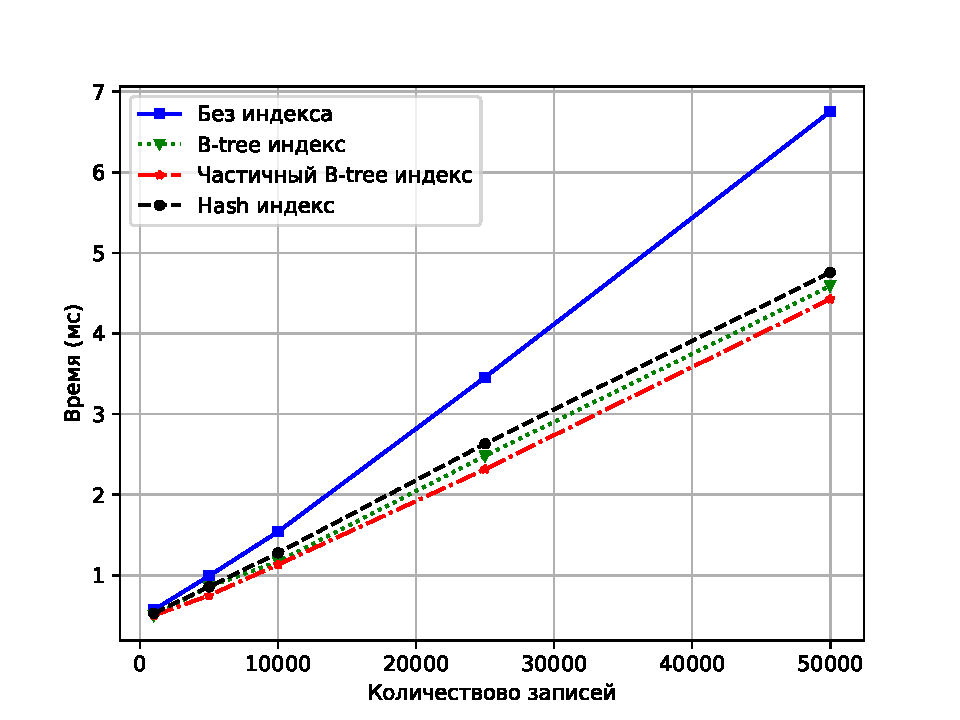
\includegraphics[width=1\textwidth, height=0.4\textheight]{research/time}
	%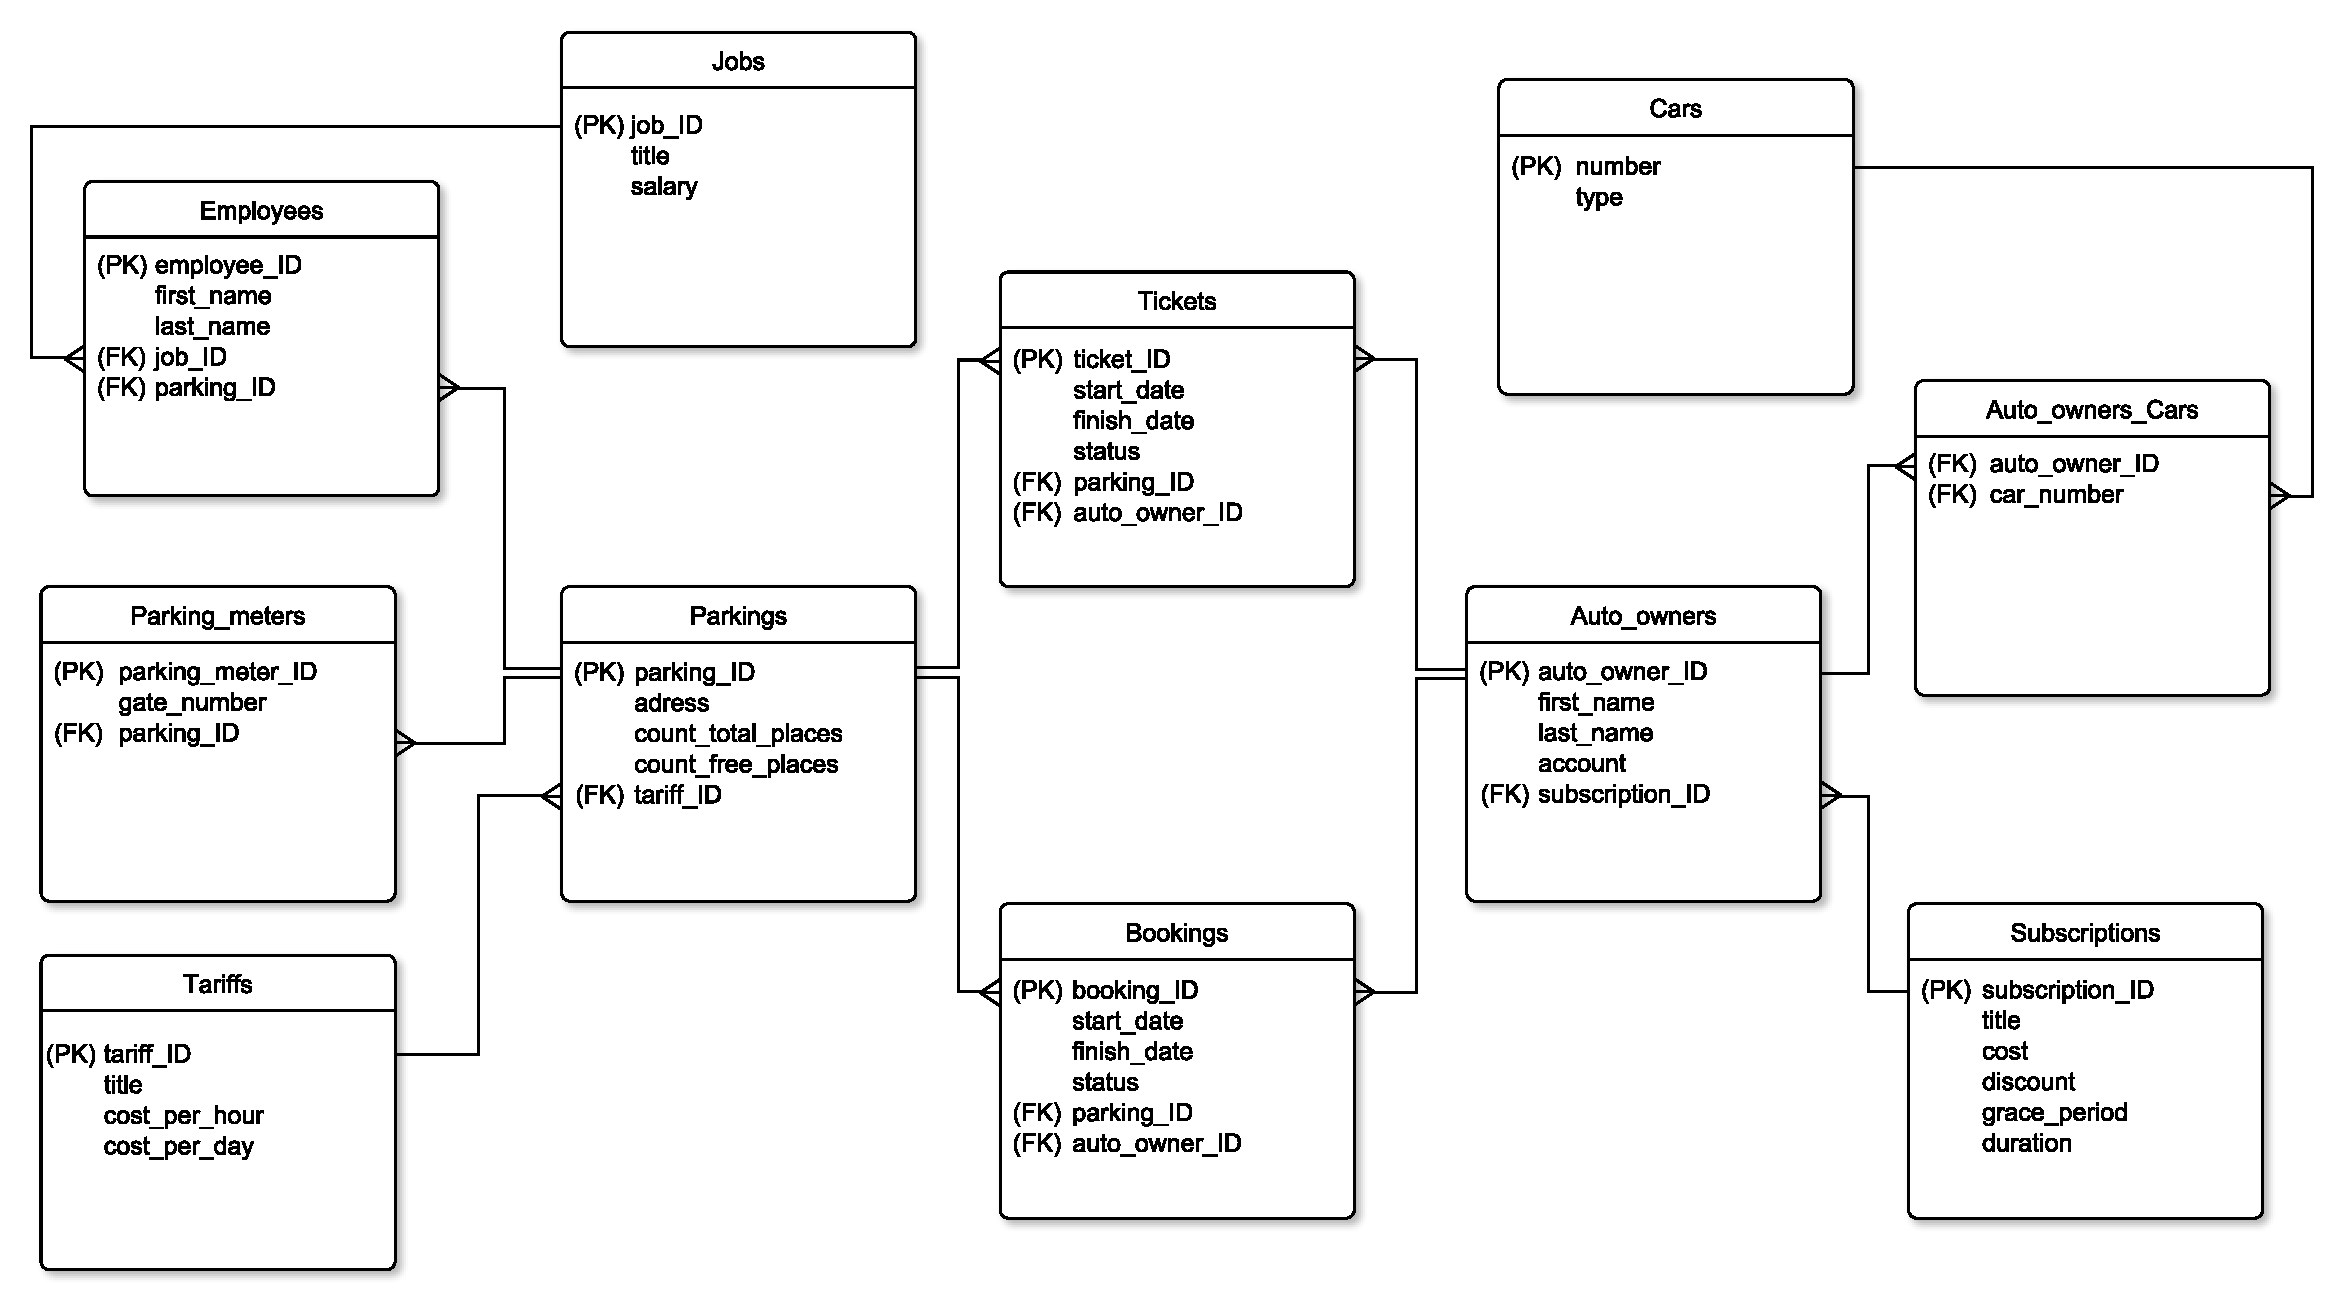
\includegraphics[height=0.5\textheight, width=0.7\textwidth]{svg/DB_diagram}
	\caption{Графики зависимости времени выполнения запроса от типа индекса и количества записей в таблице.}
	\label{fig:timeIdx}
\end{figure}
%;;;;;;;;;;;;;;;;;;;;;;;;;;;;;;;;;;;;;;;;;;;;;;;;;;;;;;;;;;;;;;;;;;;;;;;;;;;;;;;;;;;;;
В таблице~\ref{tab:memIdx} приведены результаты замеров требуемой для хранения индексов памяти.
На рисунке~\ref{fig:memIdx} представлены графики зависимости требуемой для хранения индексов памяти от типа индекса и количества записей в таблице.

\begin{table}[H]
	\begin{center}
		\begin{center}
			\caption{\label{tab:memIdx}Результаты замеров памяти в килобайтах}
		\end{center}
		\begin{tabular}{|c|c|c|c|c|}
			\hline 
			\specialcell{Количество записей\\ в таблице} & \specialcell{B-Tree \\индекс} & \specialcell{Частичный \\B-Tree индекс} & \specialcell{Hash\\ индекс}  \\\hline
		1000   & 		16 & 16 & 		64  \\ \hline
		5000   & 		56 & 16 & 		440  \\ \hline
		10000  & 		88 & 16 & 		720  \\ \hline
		25000  & 		176 & 32 & 		1560  \\ \hline
		50000  & 		336 & 32 & 		3040  \\ \hline

		\end{tabular}
	\end{center}
\end{table}

\begin{figure}[h]
	\centering
	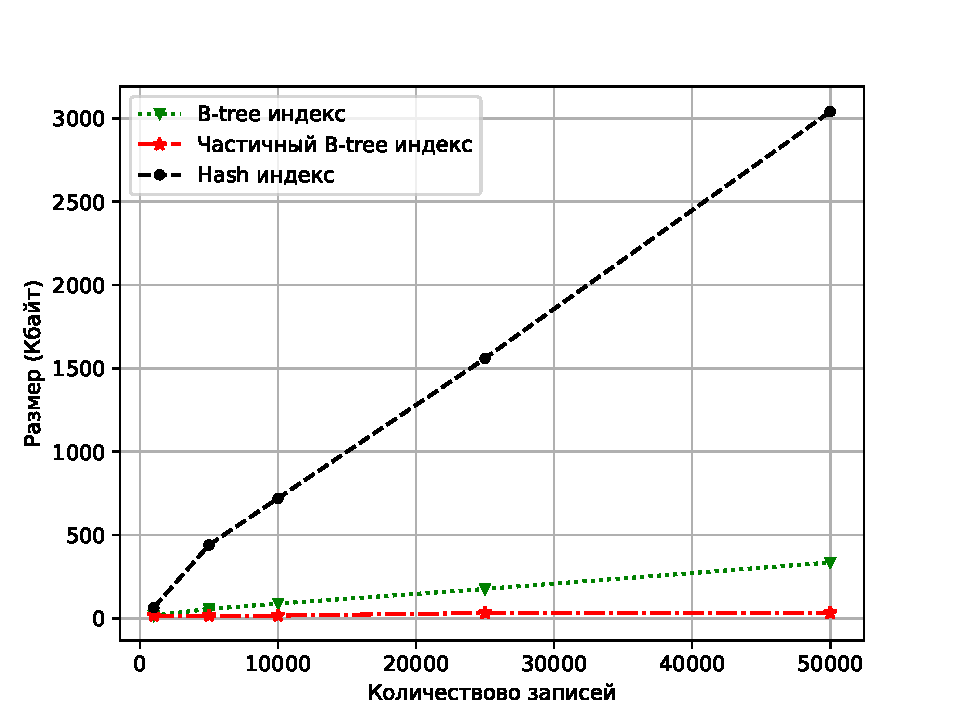
\includegraphics[width=1\textwidth, height=0.4\textheight]{research/mem}
	%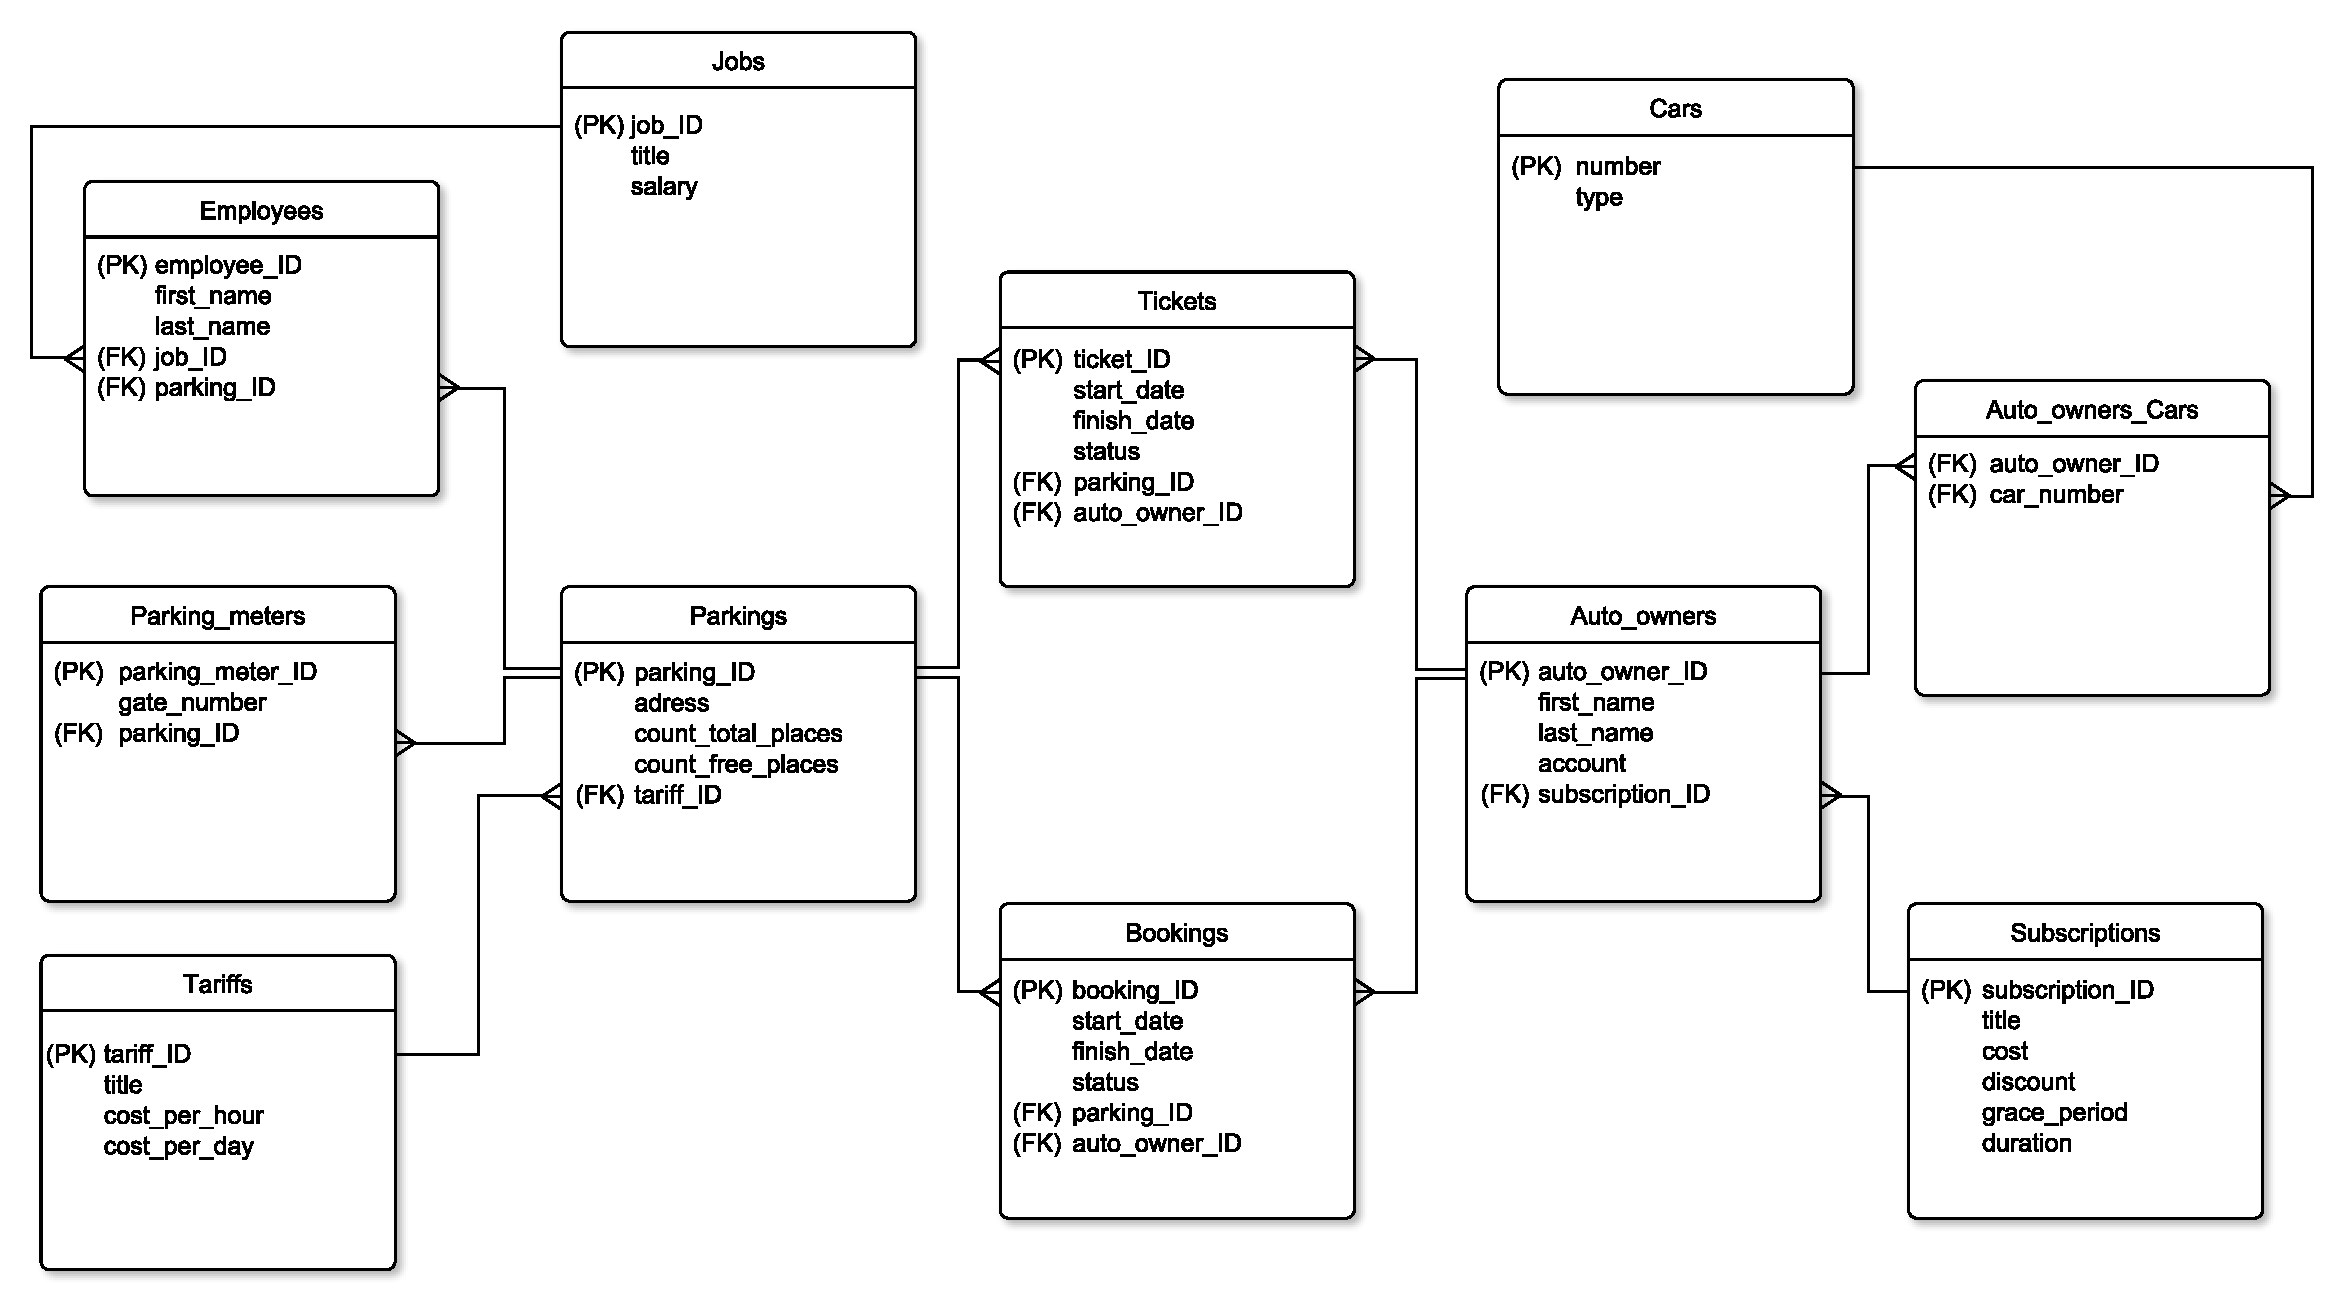
\includegraphics[height=0.5\textheight, width=0.7\textwidth]{svg/DB_diagram}
	\caption{Графики зависимости времени выполнения запроса от типа индекса и количества записей в таблице.}
	\label{fig:memIdx}
\end{figure}

%=============================================================================================
\subsect{Вывод}
Результаты исследования показали, что в ситуации, когда поиск записей осуществляется по полям, значения которых встречаются в таблице редко, лучше всего использовать частичный индекс.

Hash-индекс требует для хранения в 10 раз больше памяти, чем B-Tree индекс и в 100 раз больше, чем Частичный B-Tree индекс.Это, объясняется большим количеством коллизий, вызванным наличием всего двух возможных значений в поле типа boolean.
